\chapter{Numerical experiments}

\section{Stationary vortex preservation over long time integration}

The first numerical experiment we consider concerns the preservation of the steady-state solution of \ref{eq:gpe}. Since this solution is stationary, a natural way to assess the quality of our numerical method is to examine how much the approximate solution deviates from the initial one over long integration times.

\subsection{Uniform grid}

We now present some results from the performed experiments. The parameters used in the following simulations are: $m_x = m_y = 347$, $n_t = 450$, $t^* = 20$, $L_x = L_y = 30$.

\begin{figure}[h!]
    \centering
    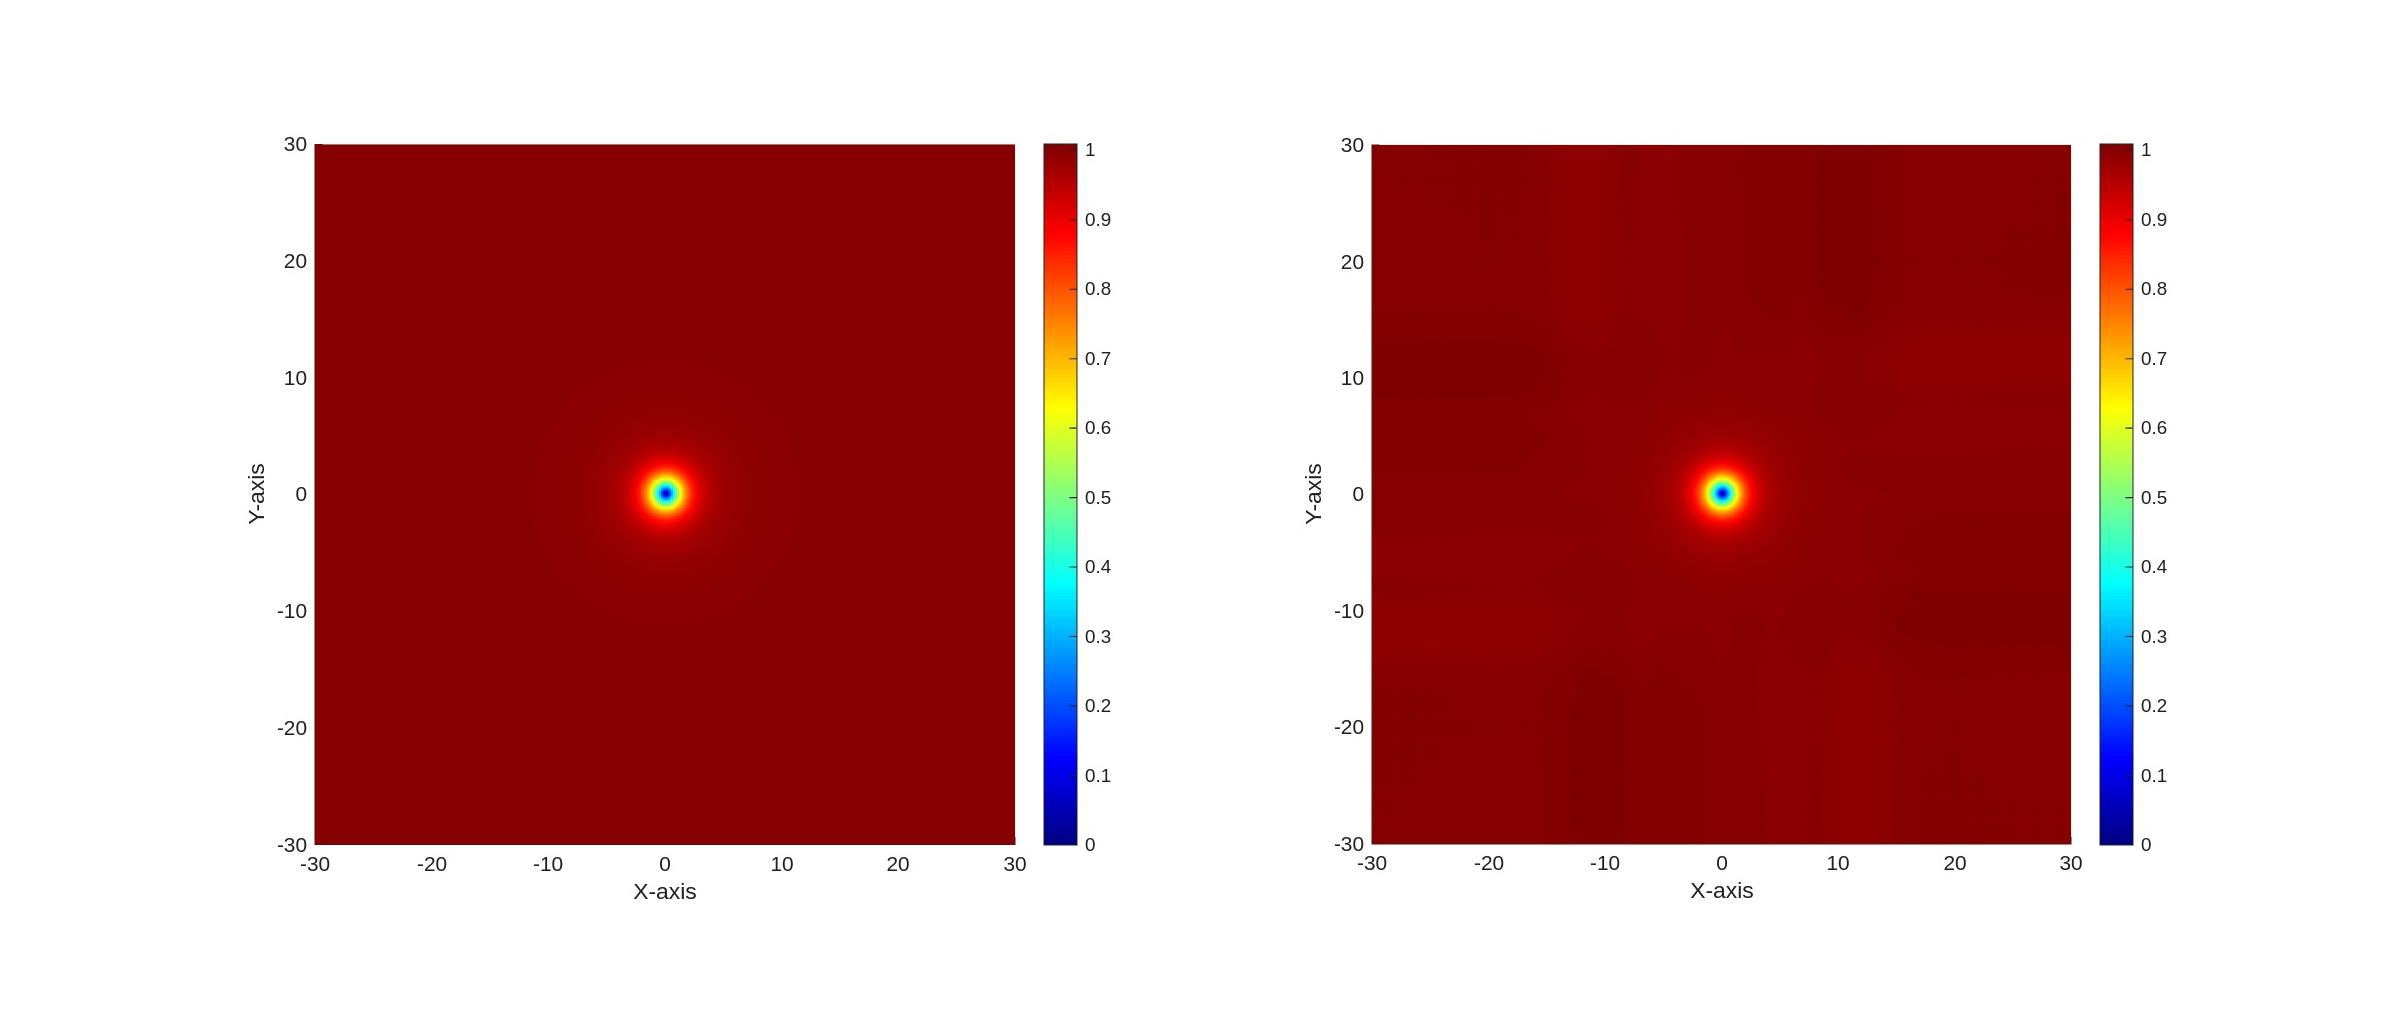
\includegraphics[width=\textwidth]{img/ltufd20t347s30L.pdf}
    \caption{$\abs{\psi_0}$ (left) and $\abs{\psi(20)}$ (right), finite differences on a uniform grid.}
\end{figure}

In this figure, we can observe that the numerical solution integrated up to $t = 20$ shows slight variations in the norm outside the vortex core. To highlight this difference more clearly, we employ an alternative colormap with a steeper gradient for values close to $1$:

\begin{figure}[h!]
    \centering
    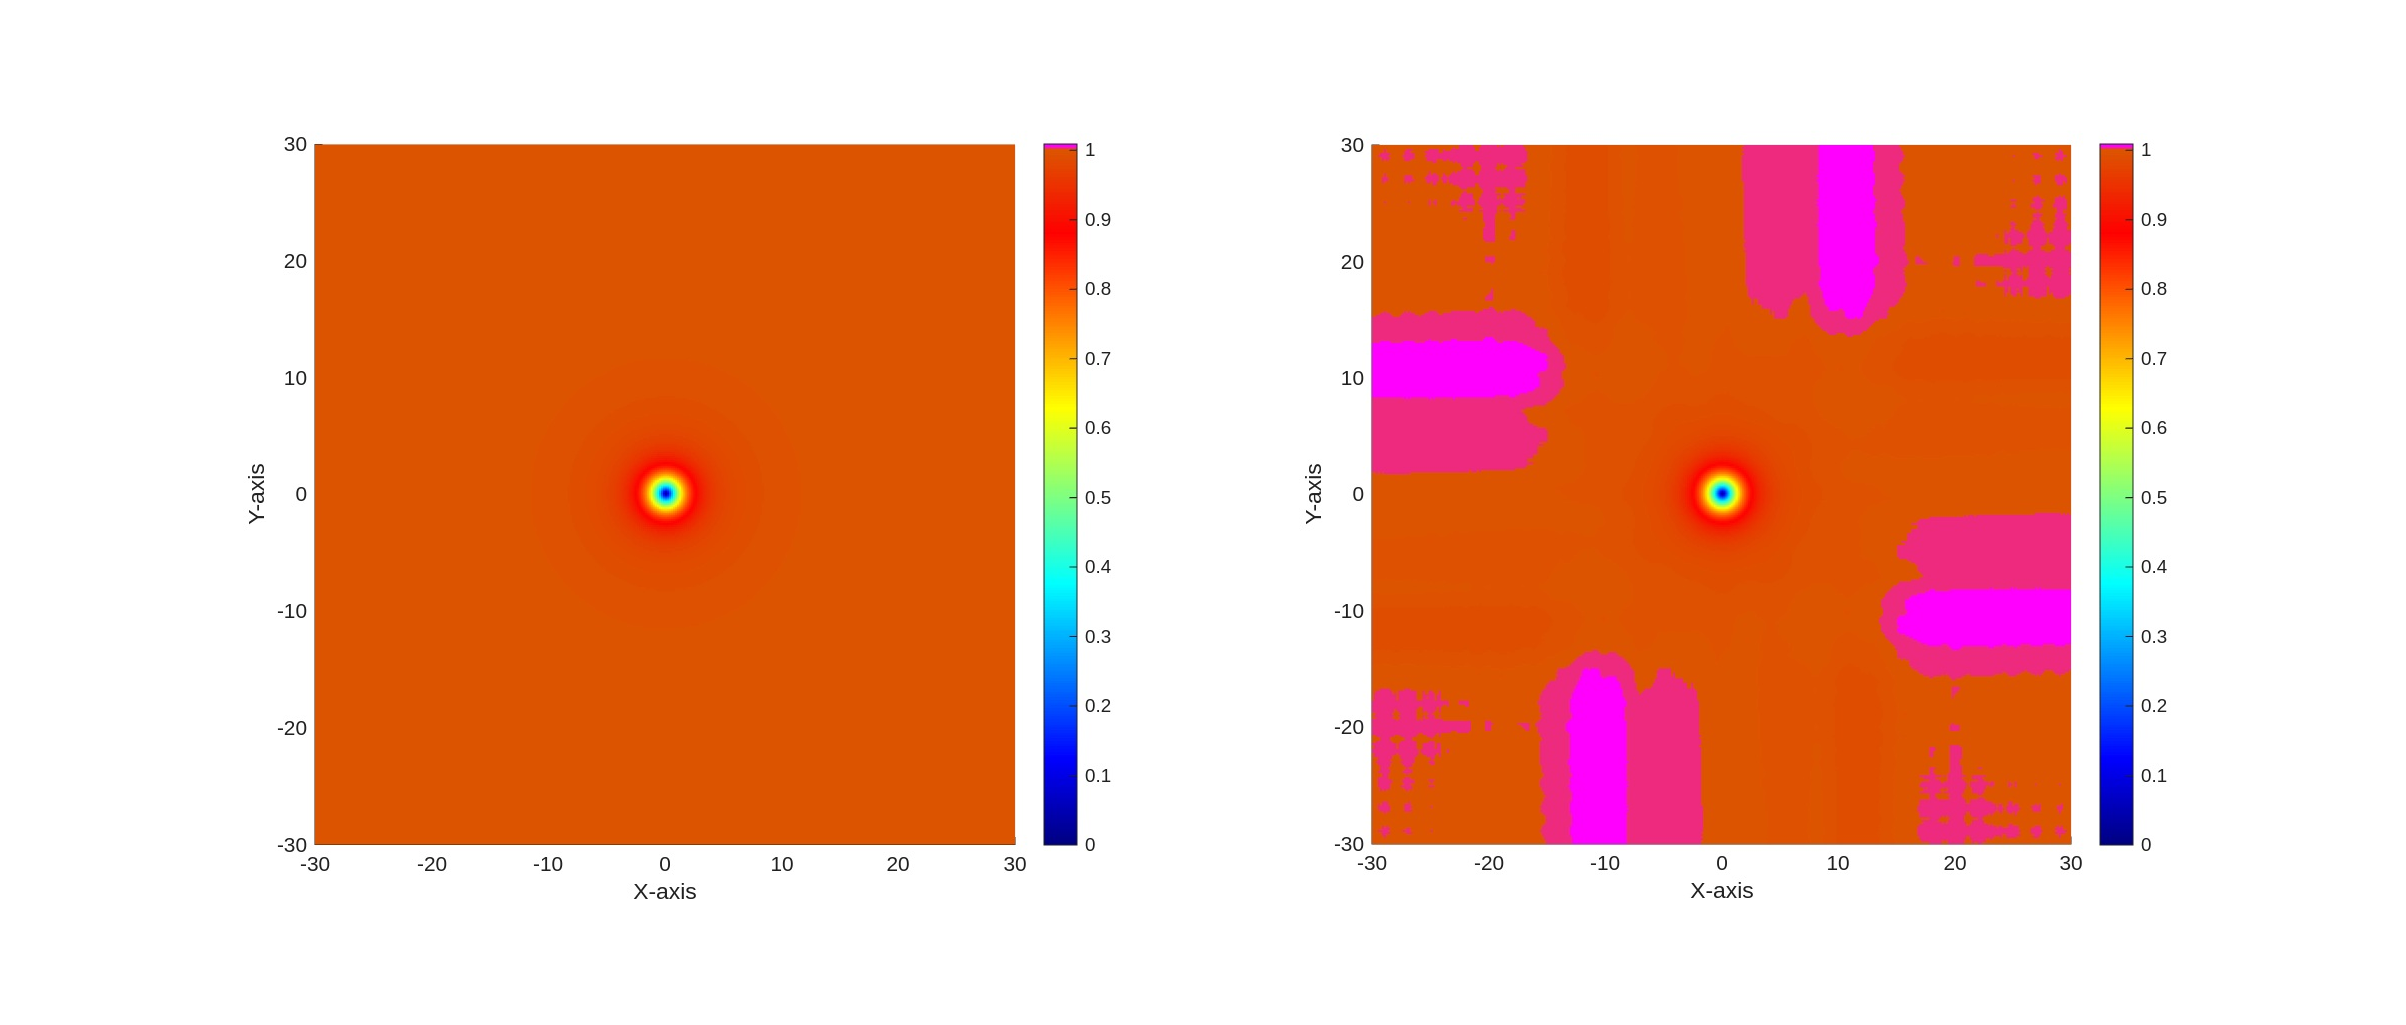
\includegraphics[width=\textwidth]{img/ltufd20t347s30L_color.pdf}
\end{figure}

We observe that the variations in the norm are localized near the limit of the domain, outside the vortex core. To highlight this, Figure~\ref{fig:vortex_center} shows the truncated domain $[-5,5]$, emphasizing the vortex center.

\begin{figure}[h!]
    \centering
    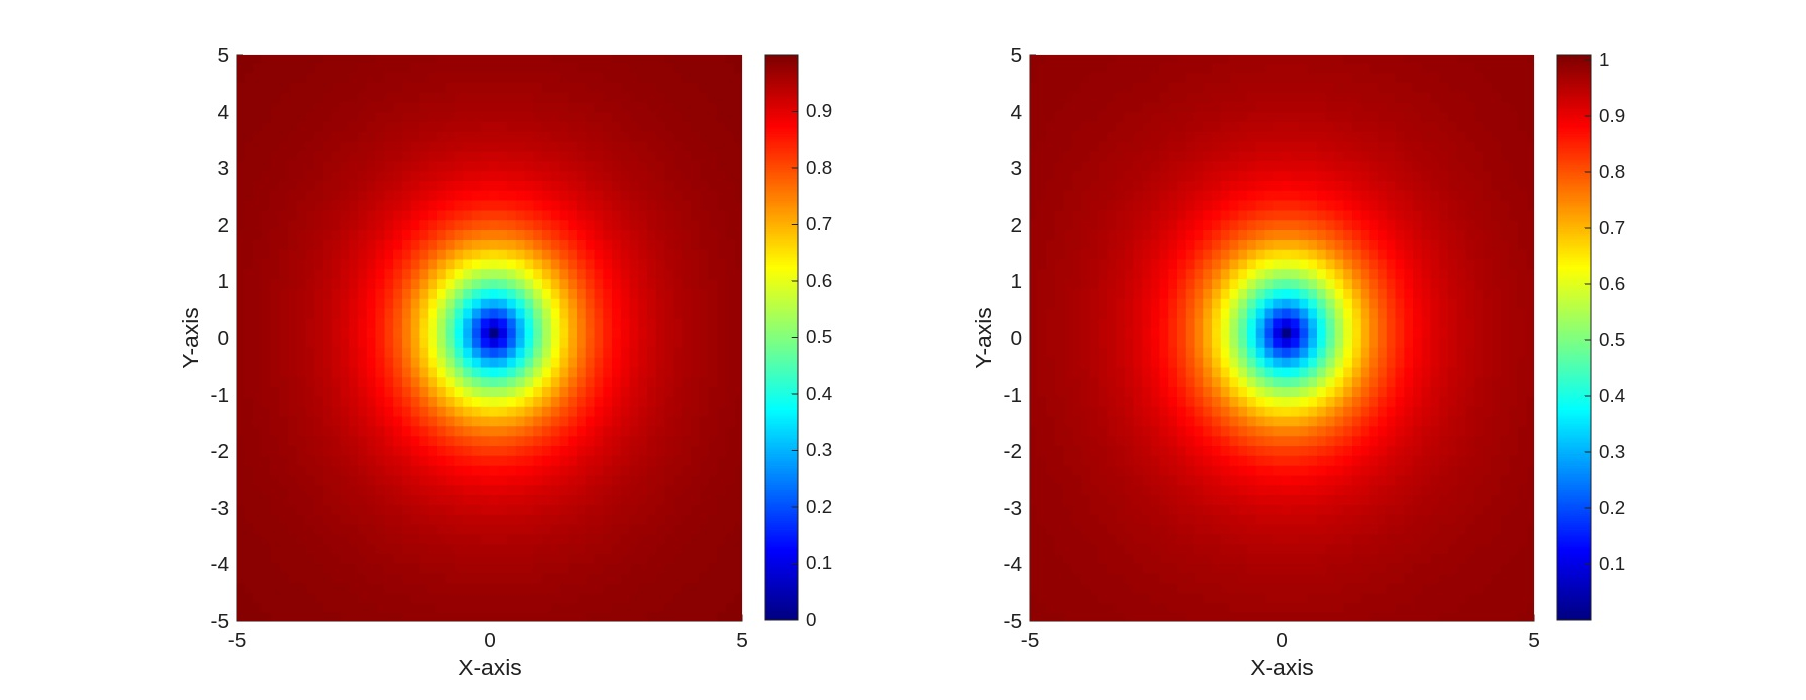
\includegraphics[width=\textwidth]{img/ltufd20t347s30L_5.pdf}
    \caption{Zoomed domain}
    \label{fig:vortex_center}
\end{figure}

From this figure, we can see that no visually appreciable variations occur near the vortex core.

\subsection{Non-uniform grid}

We now consider a non-uniformly spaced grid as described in \ref{sb:nufg}, with $\delta = h_1 = 1/50$. This results in a grid composed of 347 points per direction.

We directly report the comparison between the uniform and non-uniform grids.

\begin{figure}[h!]
    \centering
    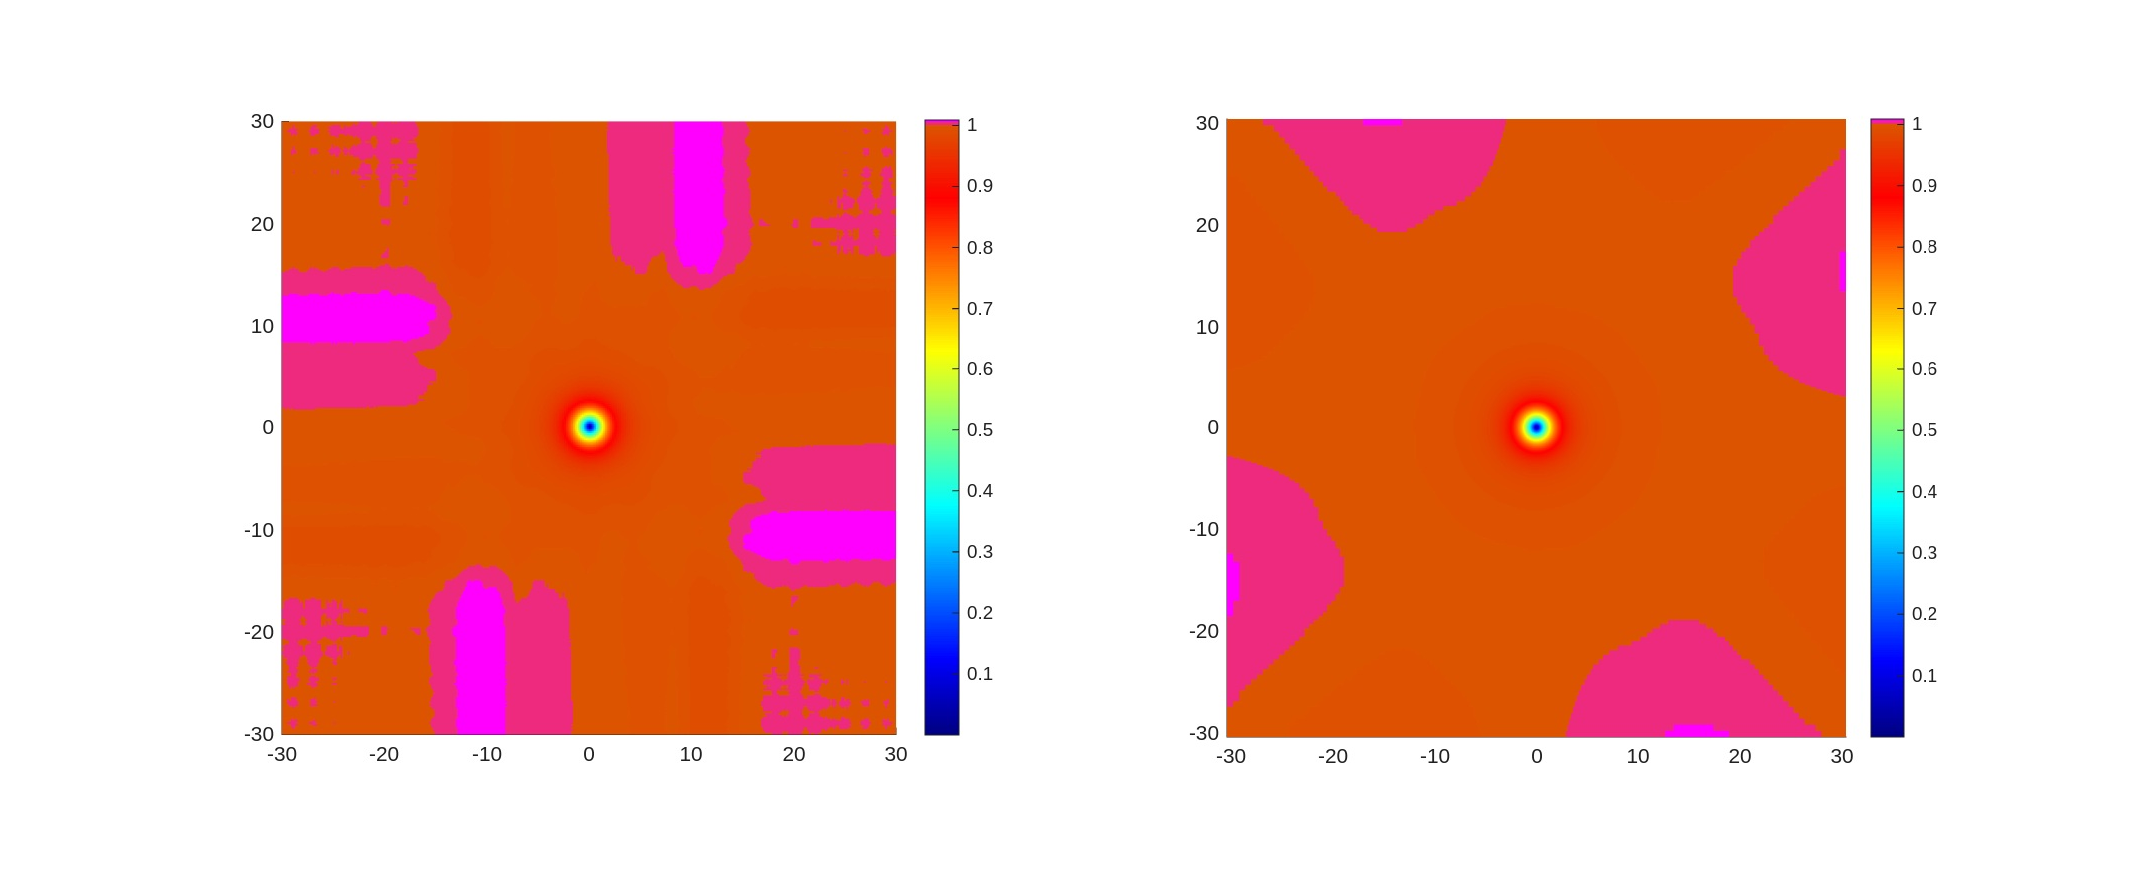
\includegraphics[width=\textwidth]{img/comparison_unfd.pdf}
    \caption{Comparison between uniform (left) and non-uniform (right) grids.}
\end{figure}

We can observe that the solution on the two grids visually differs only near the boundaries of the domain. In the case of the non-uniform grid, the deviation from the uniform grid remains smaller.

\begin{figure}[h!]
    \centering
    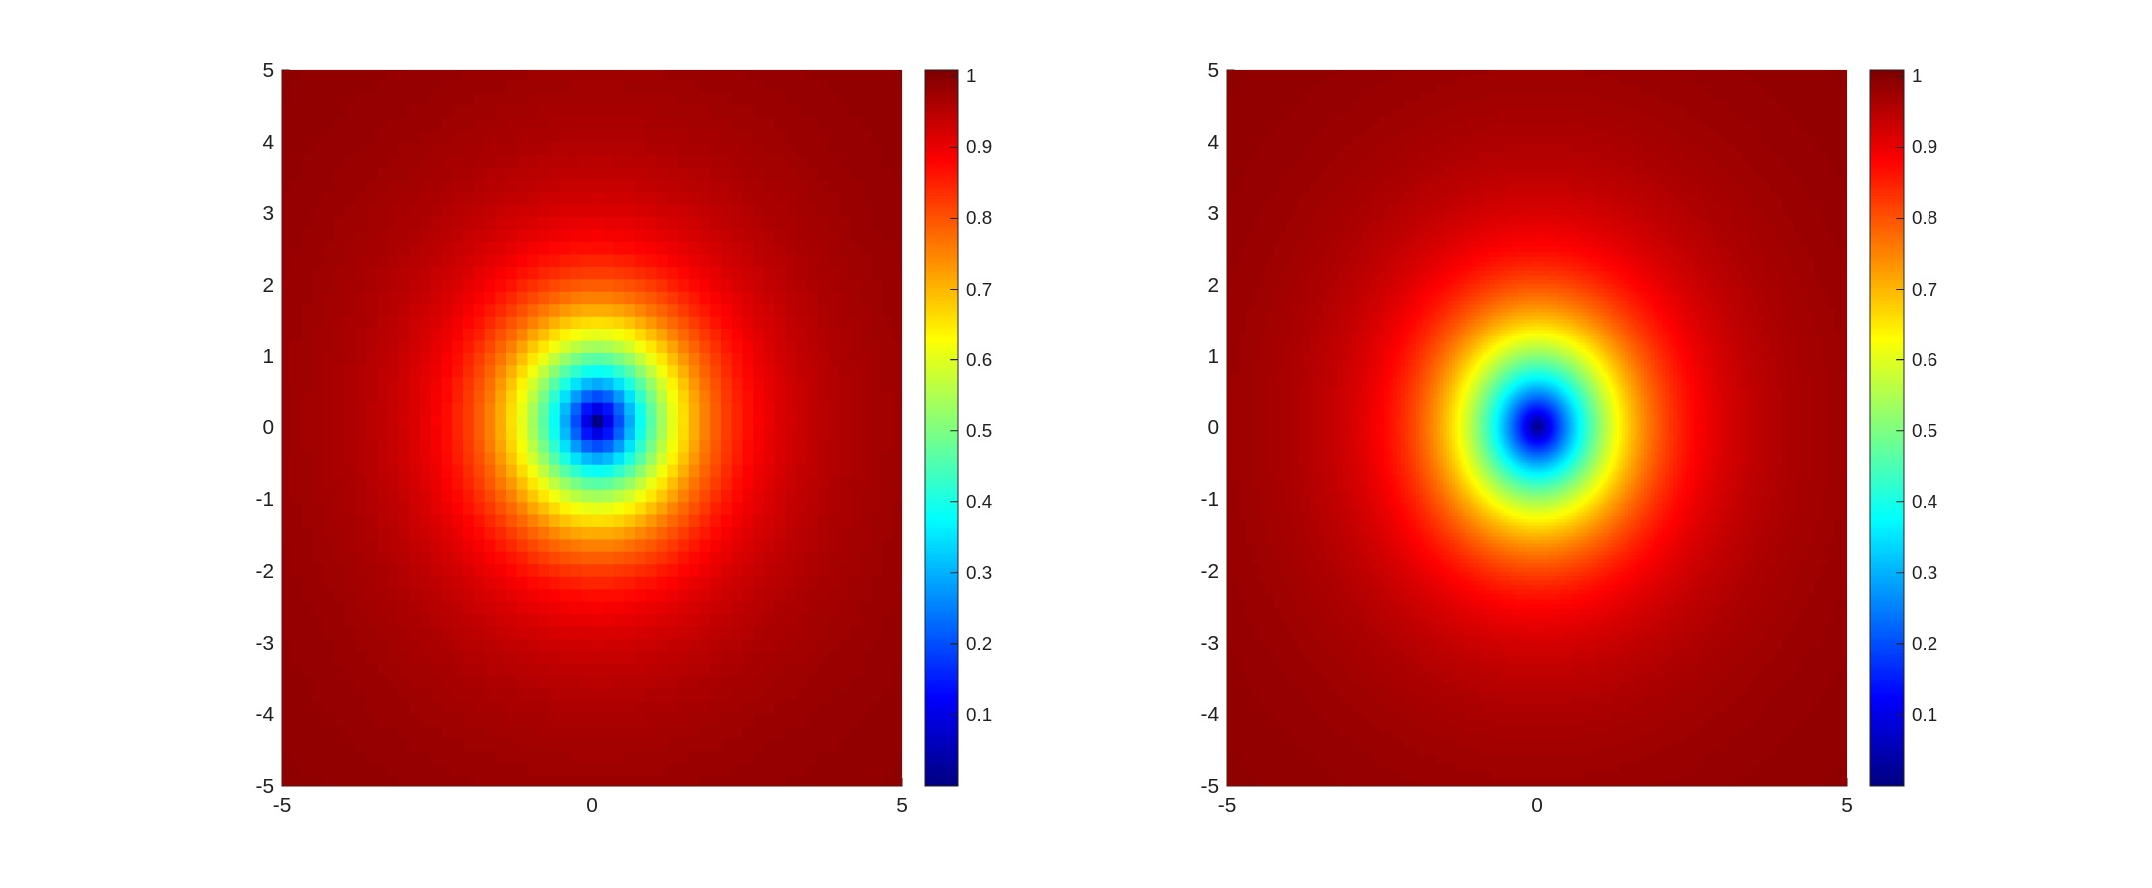
\includegraphics[width=\textwidth]{img/comparison_unfd_5.pdf}
    \caption{Zoom near the center of the domain.}
\end{figure}

Zooming into the center of the domain, no significant differences are observed. However, the refinement of the grid towards the origin in the non-uniform construction is clearly visible.

\section{Simulations of two straight vortices}

In this section, we simulate the dynamics of two interacting straight vortices. We perform experiments by imposing both concordant and opposite initial phases, and compare the different spatial discretization methods introduced so far.

\subsection{Simulation of ''marching'' vortex}

Considering the initial condition 

\[u_0 = \sqrt{\rho_1 \rho2} \exp(\ii (S_1 + S2))\]






